\section{Dominoes}

The objective is to find out where the complexity lies in the Tetris. To contribute something in this matter we will study Tetris with dominoes. From the above results it has been seen that adding more complexity in the set of pieces makes it more complicated.

Focusing on 2-\textsc{tris}, Tetris with dominoes, will help in our goal. As it can be seen in Table~\ref{tab:tt}, the variation 2-\textsc{tris-NoRotation} \clearing\ is in \npc and the only domino's problem closed.

\vspace{10px}
We will first explore two sub problems of these. We will consider the case in which all dominoes appear vertically and the case in which all pieces appear horizontally.

Then ....

\subsection{Tetris with vertical dominoes}

Using the introduced notation, the problem is $\textsc{Tetris-NoRotation}\lbrack \VD \rbrack $ both  \clearing\  and \survival. The input consist of sequence of vertical dominoes and an arbitrary sized $n \times m$ board in a contractible configuration. The initial state function used in this variation differs since the default on the initial orientation, since the pieces must come in vertical orientation.

\subsubsection{Constructible board configurations}

First we will to characterize the constructible boards with $\VD$ pieces without rotation by exploring the configuration starting from an empty board. 

Vertical dominoes consist of two vertical adjacent cells, so for an empty board any trajectory fixes the piece in the bottom row, filling $\cell[1][i]$ and $\cell[2][i]$ cells for any $1 \leq i \leq m$. The next domino can either go to an empty column or to the one before. Placing the first $m$ dominoes in unfilled columns clears the two lowest rows, and consequently the board. When a domino is placed in a non-empty column $i$, the $\cell[3][i]$ and $\cell[4][i]$ are filled, and so on, util a $\VD$ is placed in the last unfilled column. When this happens the two lowest rows are cleared and the process continues. 

So we can represent a reachable configuration of a given $n \times m$ board $B$ with a sequence of $m$ integers $(a_1, \dots, a_m)$, where

$$0 \leq a_i \leq \lceil \frac{n}{2} \rceil, \;\;\;   \forall i = 1,\dots, m$$

and $\exists i$ such that $a_i = 0$ (an empty column), with the following mapping: 

$$
\cell = \begin{cases}
   \text{filled}  & \text{if } i \leq  2a_j  \\
   \text{empty}   & \text{if } i >  2a_j
\end{cases}
$$

Each $a_i$ counts the number of vertical pieces placed in the column $i$. For example, in a $10 \times 6 $  board, the sequence $(1,2,0,4,2,3)$ defines the configuration in 
\ref{dom:vconf}.

\begin{figure}[ht]
  \centering
  \begin{subfigure}[b]{0.2\textwidth}
    \centering
    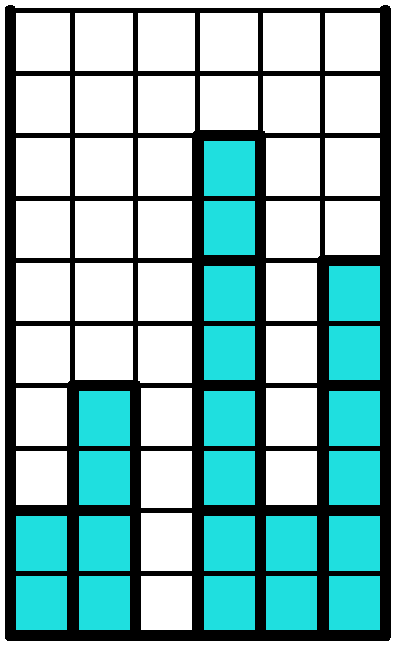
\includegraphics[width=0.9\textwidth]{pictures/dominoes/vertical_configuration.pdf}
    \caption{}
  \end{subfigure}
  \begin{subfigure}[b]{0.2\textwidth}
    \centering
    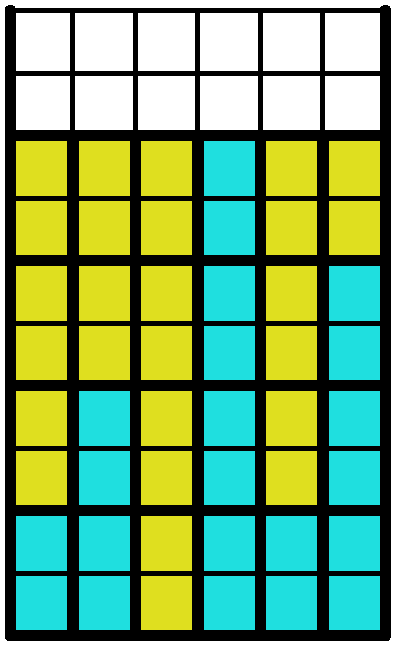
\includegraphics[width=0.9\textwidth]{pictures/dominoes/vertical_configuration_filled.pdf}
    \caption{}
  \end{subfigure}
    \caption{The $10 \times 6 $ board configuration represented by the sequence $(1,2,0,4,2,3)$, in yellow the 13 dominoes needed to clear the board.}
  \label{dom:vconf}
\end{figure}

\subsubsection{Cleaing}

In this decisional problem the input is a sequence of $k$ vertical dominoes and an $n \times m$ board with an initial configuration, that can be represented by the sequence $(a_1, \dots, a_m)$ as before. The question is: \emph{Is ther a way to clean the board after placing the $k$ pieces?}

\begin{theorem} 
$\textsc{Tetris-NoRotation}\lbrack \VD \rbrack $ \clearing\ is in \pp.
\label{dom:no-rot-vd}
\end{theorem}
\begin{proof}
    Let $B = (a_1, \dots, a_m) $ be the board representation and $k$ the length of the sequence of vertical dominoes. For every constructible board there is an empty column, so the strategy consists on placing each piece in an arbitrary empty column. 

    All the empty cells under the lowest empty row need to be filled to clean the board. Let $a_{\max}$ be the max in the board representation. Since we fill cells with dominoes, the number of dominoes $k_{\min}$ needed to clean the board is:
    $$ k_{\min} = \sum_{i = 1}^m \left( a_{\max} - a_i \right) $$

    If $k < k_{\min}$ we can't clear the board. If $k =  k_{\min}$ we can clear the board. And when $k > k_{\min}$, we can clean the board if after placing $k_{\min}$ dominoes the number of remaining pieces is a multiple of the board width, $k - k_{\min} \equiv 0 \mod m$. Since all the computations can be done in polyatomic time in respect of the input, the problem is in \pp.
\end{proof}

For boards with an even number of rows all pieces always fit inside the board. For an odd number of rows, dominoes could be placed in the top row with half of the domino inside the board and half outside. If we allow this, by changing the \emph{fix} function, the result would be the same since the same strategy works. The Figure~\ref{dom:vconf} shows, in yellow color, how the number of pieces needed to clean the board.

\subsubsection{Survival}

With the same input, the objective is to do not lose. The last proof provides a strategy to survive indefinitely. So for any number of pieces $k$ there is a way to avoid losing. Hence:
\begin{theorem} 
$\textsc{Tetris-NoRotation}\lbrack \VD \rbrack $ \survival\ is in \pp.
\end{theorem}


\subsection{Tetris with horizontal dominoes}

As before, the problem is $\textsc{Tetris-NoRotation}\lbrack \HD \rbrack $ both \clearing\ and \survival. Placing a horizontal domino fills two adjacent cells in one row or clears the row. In any constructible board each row has an even number of filled cells, so when the board width is odd row can be cleared. In this scenario the board can be cleared if the input consists on an empty board and an empty sequence of pieces. 

From now and on we assume the board has an even number of columns. Let $B$ be a board with $c$ columns. Let's divide the board in $c/2$ \emph{buckets}, a pair of consecutive columns. Then:

\begin{lemma0}   
    Not placing a domino inside a bucket makes the row unclearable.
\end{lemma0}
\begin{proof}
    Let $r$ be a row containing some dominoes. When a domino is placed in a bucket it divides the row into two parts: the cells on the left side of the domino and the ones on the right. Both parts of even length, and containing an even number of filled cells.

    In the other case the two parts have an odd length but containing an eaven number of filled cells, making them impossible to clean
    since there's no way to add an odd number of cells by placing dominoes.
\end{proof}

For example, in the Figure~\ref{dom:buckets}, the second piece occupies the second and the third bucket, making the row un-clearable. 

\begin{figure}[h]
    \centering
    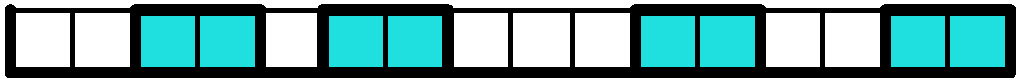
\includegraphics[width=0.2\textwidth]{./pictures/dominoes/buckets.pdf}
    \caption{A board with one partially filled row.}
    \label{dom:buckets} 
\end{figure}

We now can prove both clearing and survival problems.

\begin{theorem}
    $\textsc{Tetris-NoRotation}\lbrack \HD \rbrack $ \clearing\ is in \pp.
\end{theorem}
\begin{proof}


    The input is an $n \times m$ input board $B$, filled with a construable configuration, and sequence of $k$ dominoes $\HD$. If $m$ is odd then the board can't be cleared if $k > 0$ or the initial board isn't empty. 

    When $m$ is even we first need to check if the board is clearable. If there's only one row, checking that the row has been built by placing each piece inside a bucket determines if the row is clearable. When the board has more than one row the same happens. 

    We first group in pieces the filled cells of each row from the initial board. This can always be done because there's no way to clean \emph{"half"} piece. Then we check if each piece is placed inside a bucket. If some piece isn't placed inside a bucket the board can't be cleared. We can compute this in $\mathcal{O}(n\cdot m)$.

    Now the board can be represented with a sequence $(a_1, \dots, a_{m/2})$ of $m/2$ numbers each representing the number of dominoes placed in each bucket.

    $$
    \cell = \begin{cases}
        \text{filled}  & \text{if } i \leq  a_{2j}  \\
        \text{empty}   & \text{if } i >  a_{2j}
    \end{cases}
    $$

    With some $a_i = 0$. Let $a_{\max} = \max \{a_1, \dots \a_{m/2}$ \} be the maximum of the sequence. The minimum number of pieces needed to clear the board is:

    $$ k_{\min} = \sum_{i = 1}^{m/2} (a_{\max} - a_i )$$

    If $k < k_{\min}$ the board can't be cleared. If $k = k_{\min}$ the board can be cleared. When $k > k_{\min}$ the board can be cleared if $ k - k_{\min} \equiv 0 \mod m / 2$, sine the remaining pieces have to leave the board empty by filling rows.
\end{proof}

\begin{figure}[ht]
  \centering
  \begin{subfigure}[b]{0.3\textwidth}
    \centering
    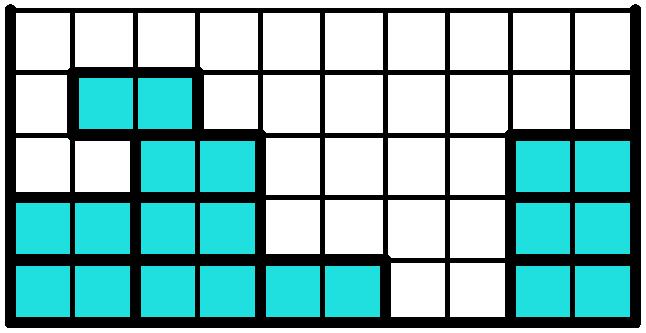
\includegraphics[width=0.9\textwidth]{pictures/dominoes/horitzonatl_configuration_1.pdf}
    \caption{}
  \end{subfigure}
  \begin{subfigure}[b]{0.3\textwidth}
    \centering
    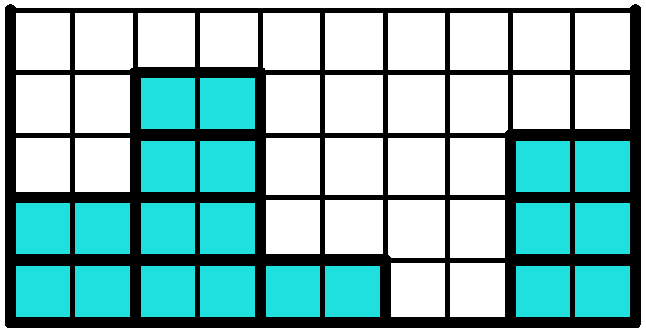
\includegraphics[width=0.9\textwidth]{pictures/dominoes/horitzonatl_configuration_2.pdf}
    \caption{}
  \end{subfigure}
  \begin{subfigure}[b]{0.3\textwidth}
    \centering
    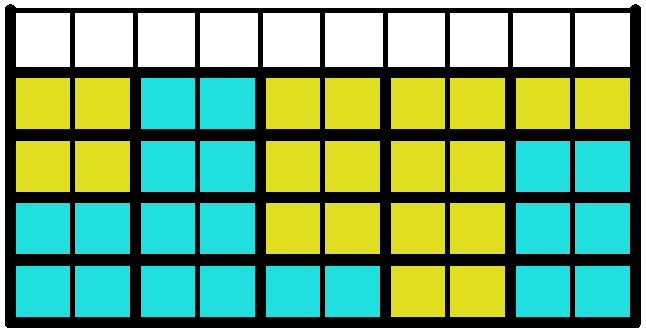
\includegraphics[width=0.9\textwidth]{pictures/dominoes/horitzonatl_configuration_3.pdf}
    \caption{}
  \end{subfigure}
  \caption{Some board configurations. In (a) the board can't be cleared because the topmost domino is placed between the first and the second bucket. In (b) the board is represented by the sequence $(2,4,1,0,3)$, it can be cleared. The minimum number of pieces to clean the board is 10, this pieces appear in yellow in (c).}
  \label{dom:horitzonatl_configuration}
\end{figure}

Figure~\ref{dom:horitzonatl_configuration} shows some examples of the above prof. Next follows the \survival. In this scenario the goal is to find a strategy to survive indefinitely...

Before the result, we need a lemma about floating pieces. A \emph{block} of dominoes is 


\begin{lemma0}
In  $\textsc{Tetris-NoRotation}\lbrack \HD \rbrack $, a board configuration with floating blocks is un-constructible.
\end{lemma0}
\begin{proof}
  Let $B$ be an $n \times m$ board with floating blocks. The width $m$ needs to be even in order to clear lines. Let $B_0, \dots, B_k = B$ be the sequence of boards that produce $B$ from an empty board $B_0$. Since $B_0$ doesn't have any floating block and $B_0$, exists a board $B_k'$ such that $B_k'$ doesn't have any floating board and $B_{k'+1}$ has one. Without loss of generality we assume $B_k$ is the first board with floating blocks. 

  By adding a domino that doesn't clear the row no floating blocks can appear, so we obtain $B_k$ by adding one domino that clears a row in $B_{k-1}$. Let $r$ be this row. If the floating block is below row $r$, clearing this row doesn't produce any effect on the block, so the block is above row $r$. If the corresponding block of cells in $B_{k-1}$ of the floating block isn't supporting on the row $r$, when the row is cleared the block would sill be connected to the rest of the configuration, so the block need to lie on the row $r$.
 
  \textbf{TO FINSH:}

\end{proof}

 
\begin{theorem}
    $ \textsc{Tetris-NoRotation}\lbrack \HD \rbrack $ \survival\ is in \pp.
\end{theorem}
\begin{proof}
    
  If the board contains a clearable row we can survive indefinitely by first clearing this row and then filling the top most row until we placed all pieces. If such a row doesn't exist, for example a board with odd width, some number $k_{\max}$ of dominoes can be placed inside board before a loss. Hence, if the input length $k$ is less or equal than $k_{\max}$ we can survive, if not we can't. The following checks if any row is clearable and computes $k_{\max}$.

  The dominoes are horizontally orientated, hence maximizing the number of dominos placed in the board consist on maximizing the number of dominoes in each row. To avoid blocking ourselves, the board will be filled starting form the bottom to top. Given a row, a \emph{hole} will be a set of adjacent empty cells that goes from a filled cell (or the left border) to another filled cell (or the right border). Each row hole has to be maximaly filled to maximaly fill a row. We reduced the problem of filling a whole board to a row hole.

  A hole needs to be reached from the top row in order to be filled. Unreachable holes are discarded, since there's no way to fill them. Lets If a hole can be reached from, 

    \begin{itemize}
      \item Fill the cells that have left and right cells filled (or outside board). 
      \item Compute the reachable space from the top row.
      \item For each row, from bottom to top:
        \begin{itemize}
          \item hasdf
        \end{itemize}
    \end{itemize} 

    Finally, 

    \textbf{TO FINSH}
\end{proof}


\subsection{Tetris Survival Without Rotation}

The problem  $\textsc{Tetris-NoRotation}\lbrack \VD \rbrack $ \survival\ can be formulated as: \emph{given an arbitrary sized board with an initial configuration and a sequence of $k$ dominoes, is there any way to play all the pieces while avoid losing?}. As is pointed in \cite{TT}, if there's a way to clear a single row then we can survive indefinitely with the following piece placing strategy: 

\begin{enumerate}
    \item Rotate the piece to be vertical. 
    \item Place the piece in any column with the two top cells empty.
\end{enumerate}

So to solve the problem we must show that, when the top row isn't empty, deciding if any row can be cleared is in \pp. 

\vspace{10px}

Before anything else we first define how dominoes a piece state is mapped into the board and how pieces move. A domino state $\piece[\VD][\theta][i][j][f]$ is mapped into: 

\begin{center}
\begin{equation}
\piece[\VD][\theta][i][j][f] \mapsto  \begin{cases}
    \{ \cell, \cell[i][j+1] \} &\text{if } \theta = 0^\circ\\
    \{ \cell, \cell[i-1][j] \} &\text{if } \theta = 90^\circ\\
    \{ \cell, \cell[i][j-1] \} &\text{if } \theta = 190^\circ\\
    \{ \cell, \cell[i+1][j] \} &\text{if } \theta = 270^\circ
\end{cases}
\end{equation}
\end{center}

It works like a clock. The piece position is the center and the second cell works as the clock handle. Figure~\ref{dom:mapping} shows the mapping for all orientations.

\begin{figure}[h]
    \centering
    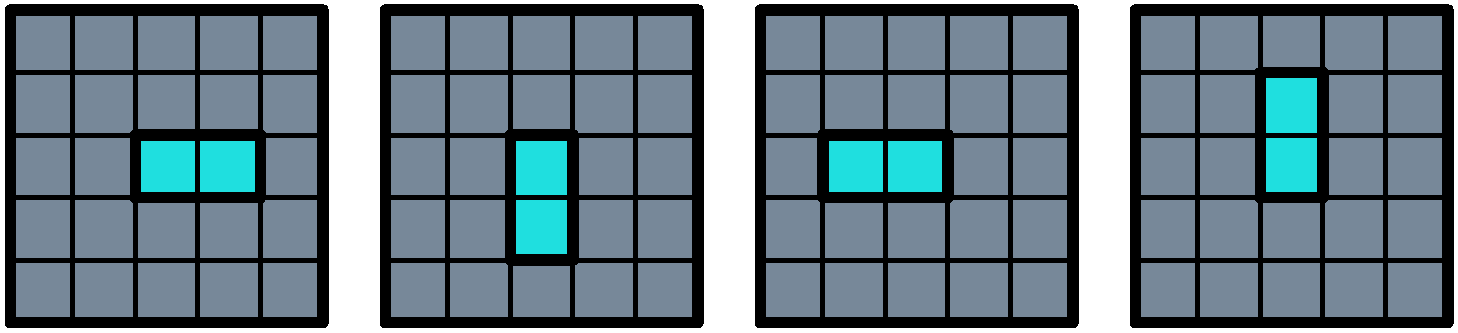
\includegraphics[width=0.6\textwidth]{./pictures/dominoes/mapping.pdf}
    \caption{The mapping of a piece placed in the center of the square and, from left to rifht, orientations $0^\circ,90^\circ,180^\circ, 270^\circ$ respectively.} 
    \label{dom:mapping} 
\end{figure}

For the moves, the usual drop and slides will be used. For the fix move we will use the \emph{partial lock rule}, witch only fixes pieces that are completely inside the board. Without this rule the strategy could be followed without the need of having the first row cleared.

For the rotation moves, the majority of modern Tetris versions use the Super Rotation System (SRS), which is the official Tetris Guideline standard for the rotation behavior of tetrominoes\cite{SRS}. When a piece is rotated, and it overlaps with a filled cell, SRS tries to place the piece in a nearby position. This is done by checking a some translations to the rotated piece. Following this idea we define a Dominoes Rotation System, DRS, with the Table~\ref{dom:rotation}.


\begin{table}[h!]
\centering
\begin{tabular}{|c || c | c || c | c ||} 
 \hline
  & \multicolumn{2}{| c ||}{ $\VD$ } & \multicolumn{2}{| c ||}{$\HD$} \\
 \hline               
 & Test 1  & Test 2 & Test 1  & Test 2 \\ 
 \hline               
 $r_+$ & $\vcenter{\hbox{
\includegraphics[scale=0.3]{./pictures/dominoes/rotation/vert_clock_1.pdf}}}$ & $\vcenter{\hbox{
\includegraphics[scale=0.3]{./pictures/dominoes/rotation/vert_clock_2.pdf}}}$  & $\vcenter{\hbox{
\includegraphics[scale=0.3]{./pictures/dominoes/rotation/horit_clock_1.pdf}}}$  & $\vcenter{\hbox{
\includegraphics[scale=0.3]{./pictures/dominoes/rotation/horit_clock_2.pdf}}}$ \\ 
 \hline                             
 $r_-$ & $\vcenter{\hbox{
\includegraphics[scale=0.3]{./pictures/dominoes/rotation/vert_anti_1.pdf}}}$ & $\vcenter{\hbox{
\includegraphics[scale=0.3]{./pictures/dominoes/rotation/vert_anti_2.pdf}}}$  & $\vcenter{\hbox{
\includegraphics[scale=0.3]{./pictures/dominoes/rotation/horit_anti_1.pdf}}}$  & $\vcenter{\hbox{
\includegraphics[scale=0.3]{./pictures/dominoes/rotation/horit_anti_2.pdf}}}$ \\ 
 \hline
\end{tabular}
\caption{The DRS rotations table. In the top rows the initial orientation of the piece: if its placed vertically or horizontally. The left columns for the rotation direction, and finally the two tests. In each picture the original piece is painted in white and the resulting piece is painted above.}
\label{dom:rotation}
\end{table}

When a piece is rotated, DRS tries to rotate the piece using the Test 1. If the resulting piece overlaps with a filled cell DRS tries with the second test. If the second test also fails the piece cannot be rotated and the move would be illegal. An example in Figure~\ref{dom:drs}.

\begin{figure}[ht]
  \centering
  \begin{subfigure}[b]{0.2\textwidth}
    \centering
    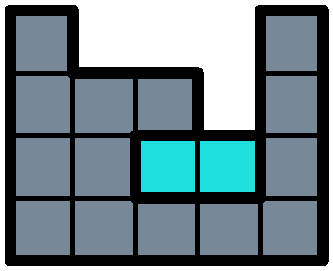
\includegraphics[width=0.9\textwidth]{pictures/dominoes/drs-1.pdf}
    \caption{}
  \end{subfigure}
  \begin{subfigure}[b]{0.2\textwidth}
    \centering
    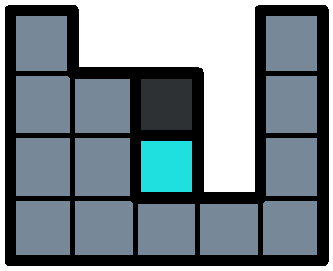
\includegraphics[width=0.9\textwidth]{pictures/dominoes/drs-2.pdf}
    \caption{}
  \end{subfigure}
  \begin{subfigure}[b]{0.2\textwidth}
    \centering
    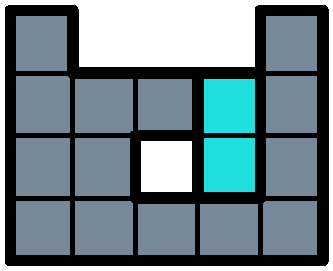
\includegraphics[width=0.9\textwidth]{pictures/dominoes/drs-3.pdf}
    \caption{}
  \end{subfigure}
  \caption{When rotating clockwise the domino in (a) DRS first ties to place it like (b), but this position isn't legal. Test 2 tries to place it in the right column which results a valid position.}
  \label{dom:drs}
\end{figure}


We will divide the problem into two: deciding when the first row can be cleared and deciding when any other row can be cleared.

\begin{lemma0}
For any $n \times m$ board, deciding whether the top row can be cleared is in \pp.
\end{lemma0}
\begin{proof}

\end{proof}

\begin{lemma0}
For any $n \times m$ board, deciding if any row, except the first one, can be cleared is in \pp.
\end{lemma0}

\begin{proof}

\end{proof}
